\documentclass{article}
%%%%%%%%%%%%%%%%%%%%%%%%%%%%%%%%%%%%%%%%%%%%%%%%%%%%%%%%%%%%%
% Lecture Specific Information to Fill Out
%%%%%%%%%%%%%%%%%%%%%%%%%%%%%%%%%%%%%%%%%%%%%%%%%%%%%%%%%%%%%
\newcommand{\LectureTitle}{L19: Shadows and Interreflections}
%\newcommand{\LectureDate}{\today}
\newcommand{\LectureDate}{March 17, 2015}
\newcommand{\LectureClassName}{CS 557}
\newcommand{\LatexerName}{Peter Henderson}
%%%%%%%%%%%%%%%%%%%%%%%%%%%%%%%%%%%%%%%%%%%%%%%%%%%%%%%%%%%%%

% Change "article" to "report" to get rid of page number on title page
\usepackage{amsmath,amsfonts,amsthm,amssymb}
\usepackage{setspace}
\usepackage{Tabbing}
\usepackage{fancyhdr}
\usepackage{lastpage}
\usepackage{extramarks}
\usepackage{chngpage}
\usepackage{soul,color}
\usepackage{graphicx,float,wrapfig}
\usepackage{afterpage}
\usepackage{abstract}
\usepackage{pgfplots}
\usepackage{caption}
\usepackage{listings}
\usepackage{minted}
\usepackage{url}

% In case you need to adjust margins:
\topmargin=-0.45in
\evensidemargin=0in
\oddsidemargin=0in
\textwidth=6.5in
\textheight=9.0in
\headsep=0.25in
\tikzstyle{cnstyle}=[domain=0:1, samples=100, ultra thick]

% Setup the header and footer
\pagestyle{fancy}
\lhead{\LatexerName}
\chead{\LectureClassName: \LectureTitle}
\rhead{\LectureDate}
\lfoot{\lastxmark}
\cfoot{}
\rfoot{Page\ \thepage\ of\ \pageref{LastPage}}
\renewcommand\headrulewidth{0.4pt}
\renewcommand\footrulewidth{0.4pt}

%%%%%%%%%%%%%%%%%%%%%%%%%%%%%%%%%%%%%%%%%%%%%%%%%%%%%%%%%%%%%
% Some tools
\newcommand{\enterTopicHeader}[1]{\nobreak\extramarks{#1}{#1 continued on next page\ldots}\nobreak
                                    \nobreak\extramarks{#1 (continued)}{#1 continued on next page\ldots}\nobreak}
\newcommand{\exitTopicHeader}[1]{\nobreak\extramarks{#1 (continued)}{#1 continued on next page\ldots}\nobreak
                                   \nobreak\extramarks{#1}{}\nobreak}

\newlength{\labelLength}
\newcommand{\labelAnswer}[2]
  {\settowidth{\labelLength}{#1}
   \addtolength{\labelLength}{0.25in}
   \changetext{}{-\labelLength}{}{}{}
   \noindent\fbox{\begin{minipage}[c]{\columnwidth}#2\end{minipage}}
   \marginpar{\fbox{#1}}

   % We put the blank space above in order to make sure this
   % \marginpar gets correctly placed.
   \changetext{}{+\labelLength}{}{}{}}

\setcounter{secnumdepth}{0}
\newcommand{\TopicName}{}
\newcounter{TopicCounter}
\newenvironment{Topic}[1][Problem \arabic{TopicCounter}]
  {\stepcounter{TopicCounter}
   \renewcommand{\TopicName}{#1}
   \section{\TopicName}
   \enterTopicHeader{\TopicName}}
  {\exitTopicHeader{\TopicName}}

\setcounter{secnumdepth}{0}
\newcommand{\ExampleSectionName}{}
\newcounter{ExampleSectionCounter}[TopicCounter]
\newenvironment{ExampleSection}[1][Example \arabic{ExampleSectionCounter}]
  {\stepcounter{ExampleSectionCounter}
   \renewcommand{\ExampleSectionName}{#1}
   \section{\ExampleSectionName}
   \enterTopicHeader{\ExampleSectionName}}
  {\exitTopicHeader{\ExampleSectionName}}

\setcounter{secnumdepth}{0}
\newcounter{ExampleBoxCounter}[TopicCounter]
\newcommand{\examplebox}[1]
  {
  % We put this space here to make sure we're disconnected from the previous
   % passage
   \stepcounter{ExampleBoxCounter}
   \noindent\fbox{\begin{minipage}[c]{\columnwidth}#1\end{minipage}}\enterTopicHeader{\ExampleSectionName}\exitTopicHeader{\ExampleSectionName}\marginpar{\fbox{\#\arabic{ExampleBoxCounter}}}
   % We put the blank space above in order to make sure this
   % \marginpar gets correctly placed.
   \vskip10pt
   }

\renewcommand{\contentsname}{{\normalsize Topics Covered}}
\renewcommand{\abstractname}{\LectureTitle\ Summary}
\renewcommand{\absnamepos}{flushleft}

\pgfplotsset{vasymptote/.style={
    before end axis/.append code={
        \draw[densely dashed] ({rel axis cs:0,0} -| {axis cs:#1,0})
        -- ({rel axis cs:0,1} -| {axis cs:#1,0});
    }
}}

%%%%%%%%%%%%%%%%%%%%%%%%%%%%%%%%%%%%%%%%%%%%%%%%%%%%%%%%%%%%%

\begin{document}
\begin{spacing}{1.1}
\newpage

% When topics are long, it may be desirable to put a \newpage or a
% \clearpage before each Topic environment
%\newpage
\begin{Topic}[Mirror Reflections \Roman{TopicCounter}]
The next texture mapping method assumes we have a mirror surface, or at least a reflectance function that contains a mirror component. Examples might be a car window or hood, a puddle on the ground, or highly polished metal or ceramic. The intensity of light reflected off each surface point towards the camera depends on what is visible from the surface in the ``mirror direction.'' We write the formula for mirror reflection:
$$r = 2n(n \cdot v) - v$$
where $v$ is the direction to the viewer and $r$ is the direction of the incoming ray. \textit{Note:} since the mirror surface is a finite distance away, the $v$ vector will typically vary along the surface regardless of whether the normal $n$ varies. Since both the surface normal and $v$ can vary along the surface, the reflection vector $r$ vector typically varies along the surface as well.

\end{topic}

\begin{Topic}[Ray Tracing \Roman{TopicCounter}]
% TODO: combine this and notes
Recall raycasting:
\begin{minted}{c}
for each pixel (x,y) {
	// 1. cast a ray through that pixel into the scene
	// 2. find the closest surface along the ray through that pixel
	// 3. compute the RGB value, based on that surface
}
\end{minted}
Ray tracing is like ray casting, but now mirror reflections are allowed. Ray tracing can be sped up using BSP trees, octrees, hierarchical bounding volumes, etc. Here's a sketch of ray tracing:

\begin{minted}{c}
for each pixel (x,y) {
	// 1. cast a ray through that pixel into the scene
	if the nearest surface is a mirror,
		repeat
			// re-cast the ray in the reflection direction
		until you hit a non-mirror surface
	else
		// compute the RGB value of the visible
		// non-mirror surface and assign that value to the pixel (x,y)
}
\end{minted}

A reflected ray uses: $\vec{r} = 2(\vec{n} \cdot \hat{v})\vec{n} - \hat{v}$. (This can be seen in Lecture 12 with mirror reflections.)

\textbf{Ray tracing does not naturally fit into graphics pipeline.}\\
Why not? Because vertex and fragment shaders only have access to a small amount of information (in particular, local scene geometry)
\end{Topic}

\begin{Topic}[Environment Mapping \Roman{TopicCounter}]
If you want real time graphics with mirror surfaces, use ``environment mapping" instead. An ``environment map" is a ``360 deg" RGB image of a scene, defined on the unit sphere centered at some scene point. We denote an environment map as $E(r)$ where r is direction of incoming ray. This CAN be done in the OpenGL pipeline.\footnote{Blinn, James F., and Martin E. Newell. ``Texture and reflection in computer generated images." 1976}

\begin{minted}{c}
for each pixel (xp,yp) {
	cast a ray through (xp, yp) to the nearest scene point (x,y,z)
	//can do this in OpenGL (get nearest scene point)

	if (x,y,z) has mirror reflectance {
		compute mirror reflection direction (rx, ry, rz)
		// copy environment map value
		// So rather than ray tracing with another cast,
		// you just have a lookup in the map
		I(xp, yp) = E(rx, ry, rz)
	}
	else{
		compute RGB using Blinn-Phong (or other model)
	}
}
\end{minted}

\subsection{Data Structures}
\subsubsection{Cube Map}
Here we represent the unit sphere of directions r by sampling the six faces of a cube\footnote{Greene, N. ``Environment mapping and other applications of world projections.'' 1986}. Each of the six faces of the cube defines a projection plane with a field of view of 90 degrees. To make a cube map using computer graphics we could render six images, each with a 90 degree field of view, and the six view directions being $\pm x, \pm y, \pm z$. The faces of the cube would be $x = \pm 1, y = \pm 1, z = \pm 1$. These (cube mapped) environment maps are pre-computed. They are OpenGL textures. So how do we index into this texture? Project r onto cube face.
$$(r_x,r_y,r_z ) = (r_x,r_y,r_z ) / \max\left\{|r_x|, |r_y|, |r_z|\right\}$$
One of the components will have value +/- 1, and this tells us which face of the cube to use. The other two components are used for indexing into that face. Need to remap the indices from [-1, 1] to [0, N) where each face of the cube map has NxN pixels.
\subsubsection{Sphere Map}
The reflection of the scene in a small mirror sphere. How much of scene is visible in the reflection off a mirror sphere? Between 180 and 360 degrees. At the top and the bottom of the sphere you can almost see right behind the sphere, but anything in between will give you in front of the sphere. So then you almost have 360, but realistically somewhere in between 180 and 360.

If you are given the reflection of a scene in a small spherical mirror, then you can compute what any mirror object looks like (if know the object's shape). Why? All you need to know is the reflection direction at each pixel and then use it to index index into the environment map defined by the given image of the sphere.
\\
How to index into a sphere map? Map $r = (r_x, r_y, r_z)$ to $(s, t)$ (points on a sphere) which is defined below. For a point on the sphere, $(x, y, z) = (n_x, n_y, n_z) = (x, y, \sqrt{1-x^2-y^2})$ by parametrization to unit circle. Then we can use this to identify $(s,t)$ coordinates with $(n_x, n_y)$.

$$\vec{n} = (n_x, n_y, n_z) = (s, t, \sqrt{1-s^2-t^2})$$

To map $r$ to $(s,t)$, assume orthographic projection, namely assume $v = (0, 0, 1)$ for all surface points. However, this is slightly incorrect because the points on top will be too far up/down. So because $\vec{r} = 2(\vec{n} \cdot \hat{v})\vec{n} - \hat{v}$. We now have $\hat{v}, \vec{n}$. Substituting for $v$ and $n$ and manipulating gives:

$$(s,t) = \frac{1}{\sqrt{r_x^2+r_y^2+(r_z+1)^2}}(r_x, r_y)$$

\textbf{What implicit assumptions are we making when using environment maps?} We assume the environment is the same for all scene points $(x,y,z)$. This essentially assumes that the environment is at infinity. Why is that wrong? Why does it not matter?

\subsubsection{Example}

Given the following scene, which would be visible to the viewer directly, through ray tracing, and then through environment mapping?

\begin{center}
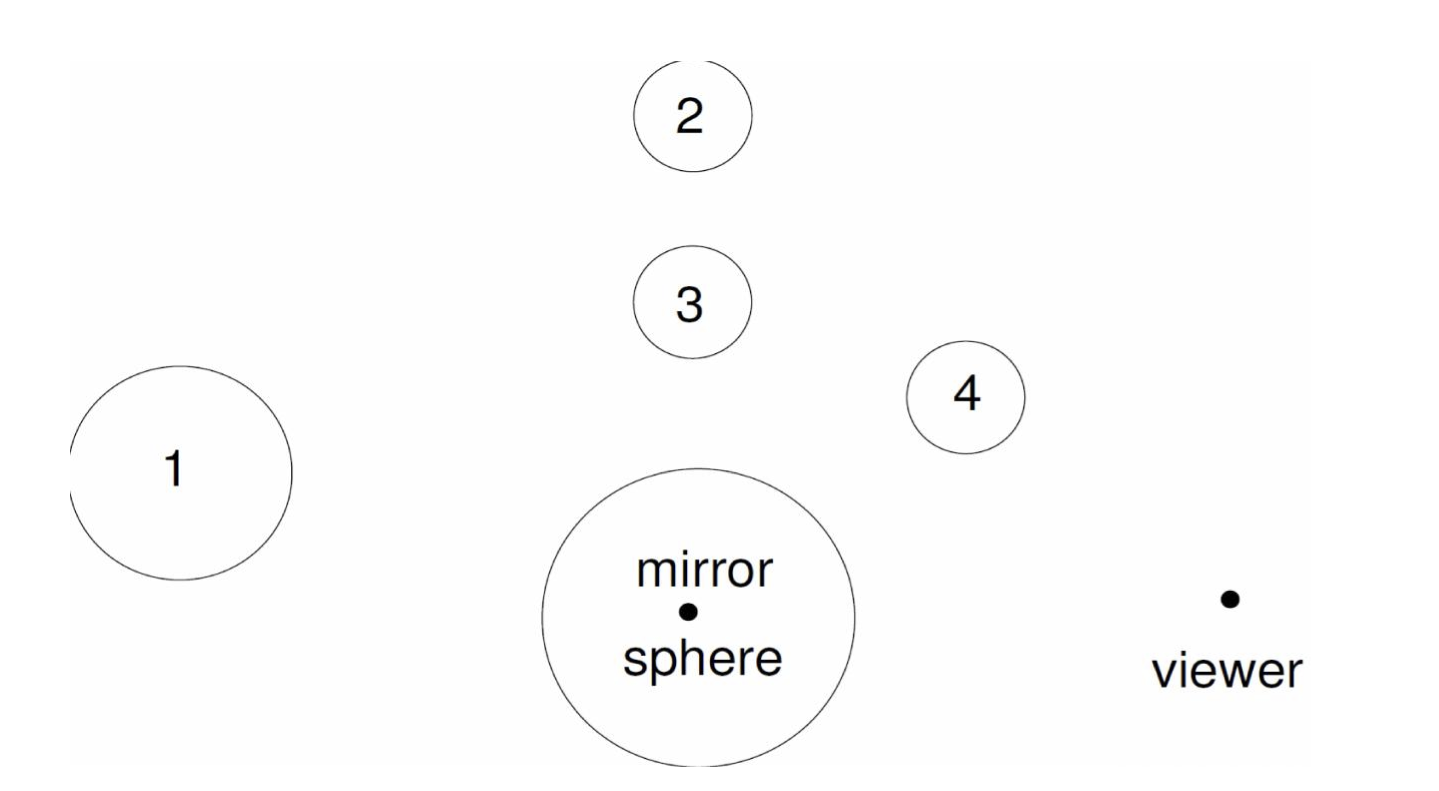
\includegraphics[scale=.34]{images/em_ex_1}
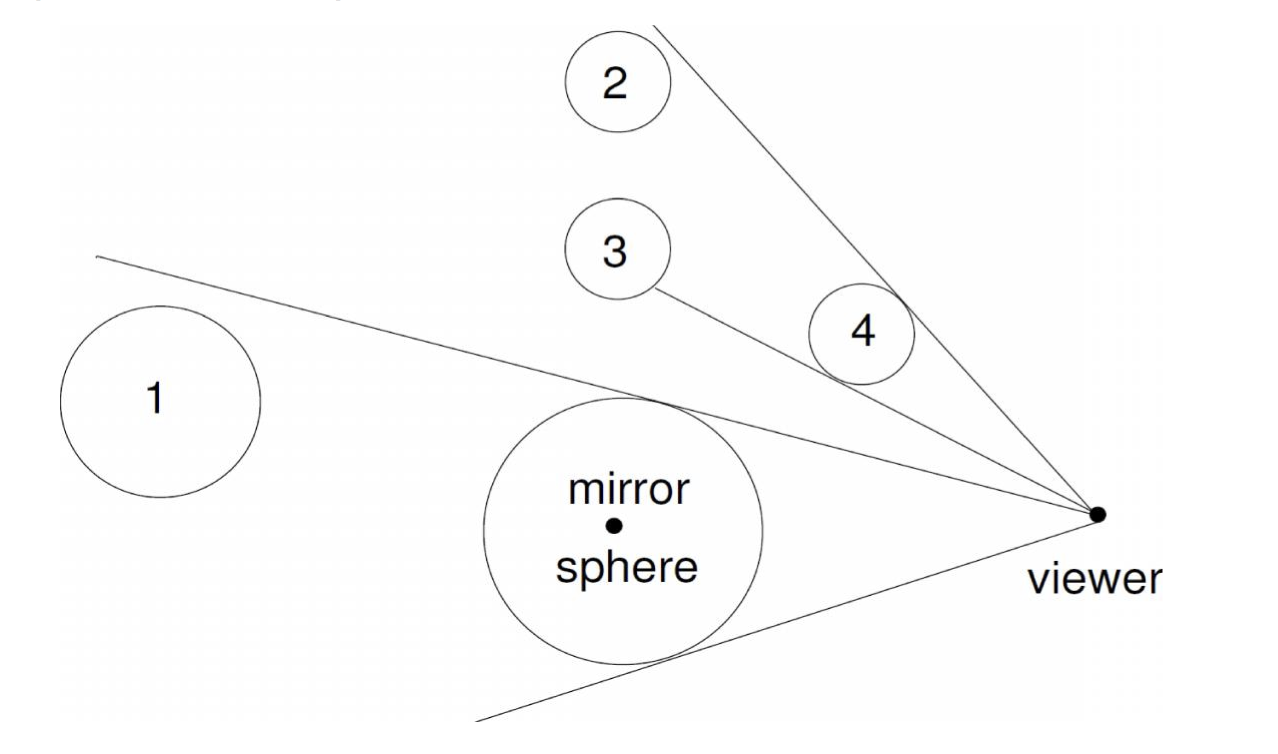
\includegraphics[scale=.34]{images/em_ex_2}
\includegraphics[scale=.34]{images/em_ex_3}
\includegraphics[scale=.34]{images/em_ex_4}
\end{center}

First, we see that the viewer can only see 3 and 4 directly. Then we see that through ray tracing 2, 3, and 4 are visible (not 1). Then through environment mapping, 1, 3, and 4 are visible but not 2. You take the tangent at the edge, and since it is in the direction of one, but you have the environment mapping at a different point. Thus you take the same direction but from a different point, giving you that one is visible. This means that around the edge of the sphere there is terrible resolution.

\subsubsection{Where in the graphics pipeline?}

Different options:
\\
\textbf{Option 1 (bad, not used)}\\\\
\textit{Vertex processor }computes the reflection vector r for each vertex, and looks up RGB values from environment map. \textit{Rasterizer} interpolates RGB values and assigns them to the fragments. Fragment processor does basically nothing.
\\\\\textit{Why is this bad?} (Hint: think of what would happen for a square mirror. It would smoothly interpolate between the values at the four corners. That's not what real mirrors do.)
\\
\textbf{Option 2 (good)}\\\\
\textit{Vertex processor} computes the reflection vector r for each vertex. \texit{Rasterizer} interpolates reflection vectors and assigns them to the fragments. \textit{Fragment processor} uses reflection vectors to look up RGB values in the environment map. Any image of a sphere can be used as an environment map.

\end{Topic}

\begin{Topic}[Refraction \Roman{TopicCounter}]
Snell's Law:
$$\frac{k_l \sin ( \theta_l)}{k_t \sin (\theta_t)} = 1$$

\begin{center}
\includegraphics[scale=.34]{images/refraction}
\end{center}

So you modify your ray through some semi-transparent object. You can use environment mapping or ray tracing to get the RGB value.
Environment mapping can be done in OpenGL 2.x and beyond using shaders.\footnote{http://3dgep.com/environment-mapping-with-cg-and-opengl/ #The_Refraction_Shader}
\end{Topic}
\end{spacing}
\end{document}